\chapter{Layout Connector Panel}

There are situations where one would connect a mobile node to the LCS bus. A good example is a cab handheld which you would like to plug in close where the session operation currently is. Even though the world moves more and more to wireless, such a connector front panel installed around the layout is not a bad idea. The panel can also be used to feature an emergency stop button and perhaps some rudimentary power status indication.

\section{Requirements}

A layout connector panel needs to provide two connectors for the LCS bus coming in and going out. The signal lines are just routed through with the exception of the power line. While these two connectors are behind the scene at the back of the front panel, two more connectors are exposed via the front panel. These are the connectors where for example a cab handheld would be plugged in. In addition to the two front panel connectors, there is an option to connect an emergency stop button. When pushed, the lines is drawn to ground and all nodes would detect the signal going low.

The power line is not directly routed to the front panel connectors. There should be an option to have an external power supply to provide the power to the nodes. It depends on the total power consumption we expect on the LCS bus. The central source will be a power supply that delivers about one amp to the lCS bus. To power a couple of handhelds or small sensors nodes, would not be a problem. As the power demand grows, a separate power supply such as shown on the schematic below will deliver the necessary power.

\section{Implementation}

The following schematic shows the LCS connector panel schematic. The upper part contains all the connectors and the option to connect an external power source to the front panel. The lower part shows a simple power supply, which could directly be hosted on the connector PCB.

\begin{figure}[h]
    \centering
    %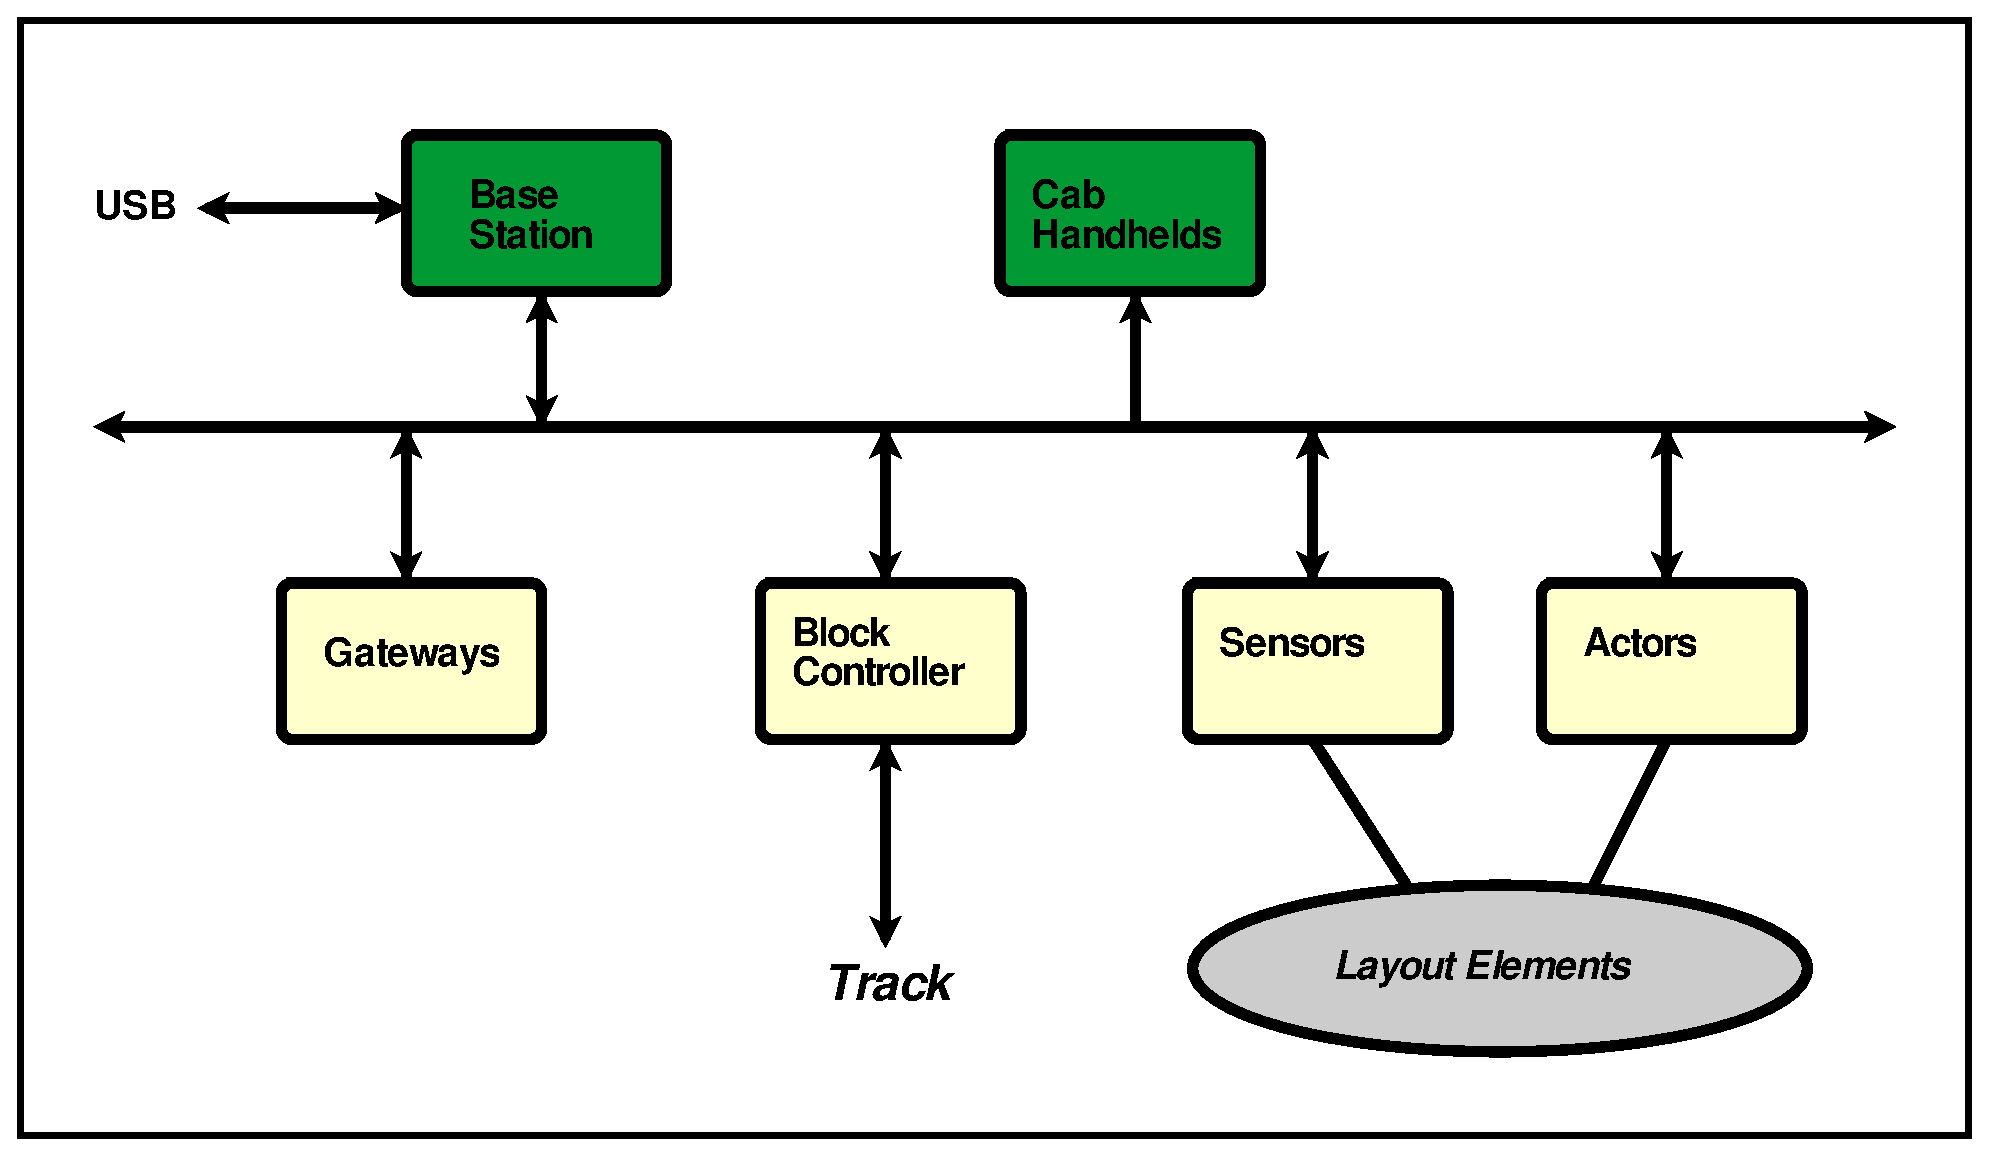
\includegraphics[page=1, width=\textwidth]{./figures/Schematic_LcsNodes-Layout-Overview.pdf}
    % !\href{./Schematics/Schematic_LcsNodes-Layout-Front-Panel.png }{Schematic_LcsNodes-Layout-Front-Panel.png}
\end{figure}

\section{Summary}

This rather short chapter shows how a layout connector panel could be designed. Such panels are placed on strategic points around the layout. Besides connecting mobile devices to the LCS bus, there is also the option to feed these devices with an external power.  The panel is also a good spot to place emergency stop buttons around the layout.  The current panel is just connector routing panel.  Additional status information for power on, bus activity, and so on could also be put onto such a panel. However, anything more complex would require to put some controller logic on the panel as well.

